\documentclass{article}
\usepackage[T1]{fontenc}
\usepackage[utf8]{inputenc}
\usepackage{indentfirst}
\usepackage{float}
\usepackage{natbib}
\usepackage{graphicx}
\usepackage{grffile}
\usepackage{epsfig}
\usepackage{soul}
\usepackage{pdflscape}
\usepackage{hyperref}
\usepackage[a4paper, total={16cm, 25cm}]{geometry}

\title{
\vspace{-10mm}
\hline
\vspace{5mm}
\Huge Nutr.io - Multi-platform application for diabetics' nutritional choices\\
\Large Project's Proposal\\
\Large Instituto Superior de Engenharia de Lisboa\\
\Large Licenciatura em Engenharia Informática e de Computadores
\vspace{5mm}
\hline
\vspace{-10mm}
}
\date{March 16, 2020}

\begin{document}

\maketitle

\section{Project Group and Tutor}
    \begin{itemize}
        \item Group:
            \begin{itemize}
            \item Pedro Miguel Sequeira Pires
            \begin{itemize}
                \item Number: 42206
                \item Phone: +351 965 621 741
                \item Email: A42206@alunos.isel.pt
            \end{itemize}
        \end{itemize}
        \begin{itemize}
            \item Miguel Filipe Paiva Luís
            \begin{itemize}
                \item Number: 43504
                \item Phone: +351 969 567 540
                \item Email: A43504@alunos.isel.pt
            \end{itemize}
        \end{itemize}
        \begin{itemize}
            \item David Alexandre Sousa Gomes Albuquerque
            \begin{itemize}
                \item Number: 43566
                \item Phone: +351 968 702 017
                \item Email: A43566@alunos.isel.pt
            \end{itemize}
        \end{itemize}
    \end{itemize}
    \begin{itemize}
            \item Tutor:
            \begin{itemize}
                \item Fernando Miguel Gamboa de Carvalho
                \begin{itemize}
                    \item Email: miguelgamboa@outlook.com
                \end{itemize}
            \end{itemize}
        \end{itemize}
    

\section{Introduction}

The idea that every field of study can be digitalized in order to ease monotonous tasks is continuously growing in the modern world. Our project aims to tackle the field of Type 1 diabetes, given its growing prevalence in the world\cite{world}.\\

One of those monotonous tasks is the count and measurement of carbohydrates in meals used to administer the correspondent amount of insulin, along with their blood levels, to maintain a healthy lifestyle. A task that heavily relies on having access to food databases\cite{idf} and realize of how many portions a meal has - usually by using a digital balance or doing estimations.\\

Eating in restaurants is the perfect example that showcases a gap in this field, that our project, 
Nutr.io, aims to fill.  Most nutritional applications do not provide data for restaurants' meals, such as MyFitnessPal\cite{myfitnesspal}, nor does the user bring his digital balance from home - resulting in a faulty carbohydrate count and therefore the administration of an incorrect insulin dose.\\

The main goal of this project is to design a system that offers a way to facilitate difficult carbohydrate measurement situations, like in restaurants. To that end, a system that stores meals' nutritional information will be developed, where users can use and calibrate its data with their feedback.\\

\textbf{Keywords:} Diabetes; Nutrition; Contribution.

\subsection{Goals}

Given the gaps stated in the Introduction, Nutr.io aims to develop a system that offers to the users the carbohydrates values of meals available in restaurants. The information is collected from external APIs and gradually calibrated by using other sources, such as users' feedback. All data gathered from these sources is stored in an internal system's database.\\

This project aims to achieve these goals by fulfilling the following requirements at the end of this project: 

\begin{itemize}
    \item Use external APIs to obtain data from meals and restaurants;
    \item Maintain a database that contains the baseline nutritional values and their calibration provided by other sources;
    \item Obtain baseline nutritional information about meals of any given restaurant. (Even when restaurants do not supply their menus to any API);
    \item A contribution system that uses data from different kind of sources to calibrate a meal's nutritional information for a given restaurant. Those sources may include:
        \begin{itemize}
            \item System's community (mandatory objective);
            \item Nutritionists (optional objective)
            \item Restaurant owners (optional objective)
        \end{itemize}
    \item Implement registration and authentication support, so that authenticated users can contribute to the community.
\end{itemize}

\subsection{Lower Priority Goals}

Due to the diversity of features that must be implemented, the following objectives were also considered but marked with a lower priority, making their completion dependent on the state of the project:

\begin{itemize}
    \item Extend the project's contribution system by adding the following features:
    \begin{itemize}
        \item Allow authenticated users to also submit custom dishes for a given restaurant; and new restaurants, if the application's API fails to provide it;
        \item A point-based system, similar to \textbf{StackOverflow}\cite{stackoverflow}, where user's contributions can be downvoted or upvoted by authenticated users.
    \end{itemize}
    \item Reward custom labels to users, which can be seen on their profiles, based on their points and contributions;
    \item Establish minimum requirements, such as number of points, for community contributions;
    \item Allow users to locally save meals and their information, so that it can be read in an offline mode;
    \item Add support to compose a custom dish out of various ingredients, which can be saved locally or added to a restaurant's list of dishes;
    \item Add support for multi-platform synchronization regarding user's local data;
    \item Implement additional quality of life features for both mobile and browser-based applications, such as a dark mode.
\end{itemize}

\section{Analysis and approach}

This project will be deployed using \textbf{Heroku}\cite{heroku} and coded in four system components - an HTTP-based API, a relational-based database, a mobile application and a browser-based application; which can be analyzed in figure 1:\\

\begin{figure}[H]
    \centering
    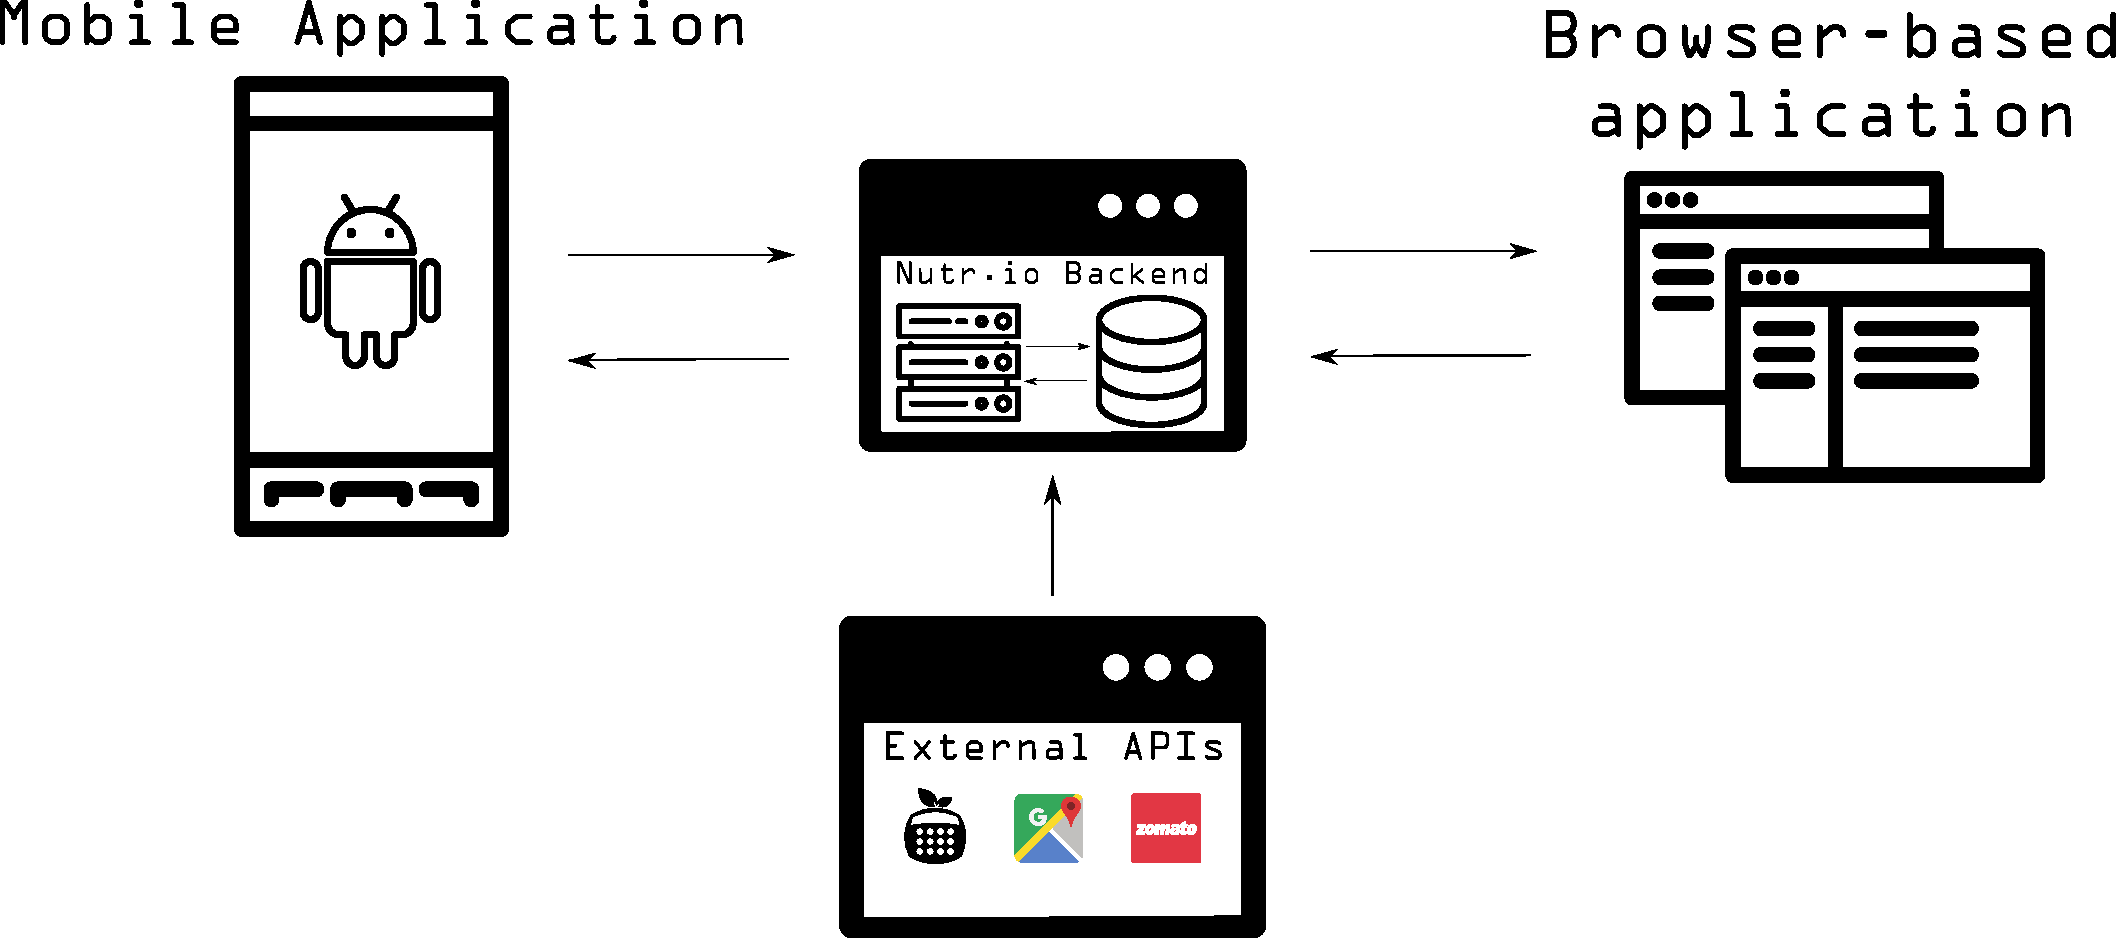
\includegraphics[scale=0.3]{pictures/Nutr.io System Components.pdf}
    \caption{Nutr.io System Components (Vector format)}
    \label{fig:Nutr.io System Components}
\end{figure}
The HTTP-based API will be implemented in Kotlin using the Spring framework to provide endpoints that allow the users to read and write data. Said data can be the following:

\begin{itemize}
    \item Restaurants' cuisines, which are obtained from external APIs, such as \textbf{Google Places}\cite{googleplaces}, \textbf{Zomato}\cite{zomato} and \textbf{Yelp}\cite{yelp}, which are read by users; 
    \item Restaurants' meals, which are obtained from the external APIs mentioned above and the system's database, seeing as the community can write their own meals;  
    \item Meals' nutritional values, where their baseline values are obtained from nutritional APIs, such as \textbf{Nutritionix}\cite{nutritionix} and additional calibration done by the community is saved to the system's database.
\end{itemize}

Taking into consideration the complexity of the previously mentioned data and how they relate to each other, a relational-based database approach was chosen over a non-relational one.\\

The mobile application will be targeted for Android and implemented using Kotlin.\\

Finally, the browser-based application will be implemented using the \textbf{React Framework}\cite{react} in a single-page application approach since we aim to offer a rich user interface with many features, and its fast and responsive properties.\cite{singlepage1}\cite{singlepage2}\\

\section{Risks}

The main risk to the project is the heavy dependency in obtaining restaurants' meals. If no external API is capable of providing accurate and reliable data (such as \textbf{Zomato}\cite{zomato}, which despite offering an endpoint for restaurants' daily menus, not enough owners use this feature \cite{zomato1}\cite{zomato2}\cite{zomato3}), alternate approaches must be taken - such as assigning an immutable list of meals to cuisines, used as a default for restaurants that do not provide their meals.\\

The other significant risk is that the project relies on skills that the group has not acquired yet and that are being taught in ISEL's courses (namely DAW). If said courses suffer a delay in providing their knowledge, then the scope of the implementation must be delayed or restricted.\\

Lastly, due to the recent outbreak of \textit{COVID-19} and the resultant pandemic situation, the group expresses concerns about any possible setbacks that the virus can cause. These setbacks could include canceled meetings with our tutor, canceled classes (reinforcing the previously mentioned risk) and delays in our project plan due to a member being infected. Virtual meetings and calls should be considered as alternatives in order to maintain a steady workflow and solve this issue. 

\section{Project's Schedule}

Detailed plans will be produced as part of the individual project report, but the following project's schedule was developed to highlight any milestones that appear achievable from initial planning:\\

\begin{figure}[H]
    \centering
    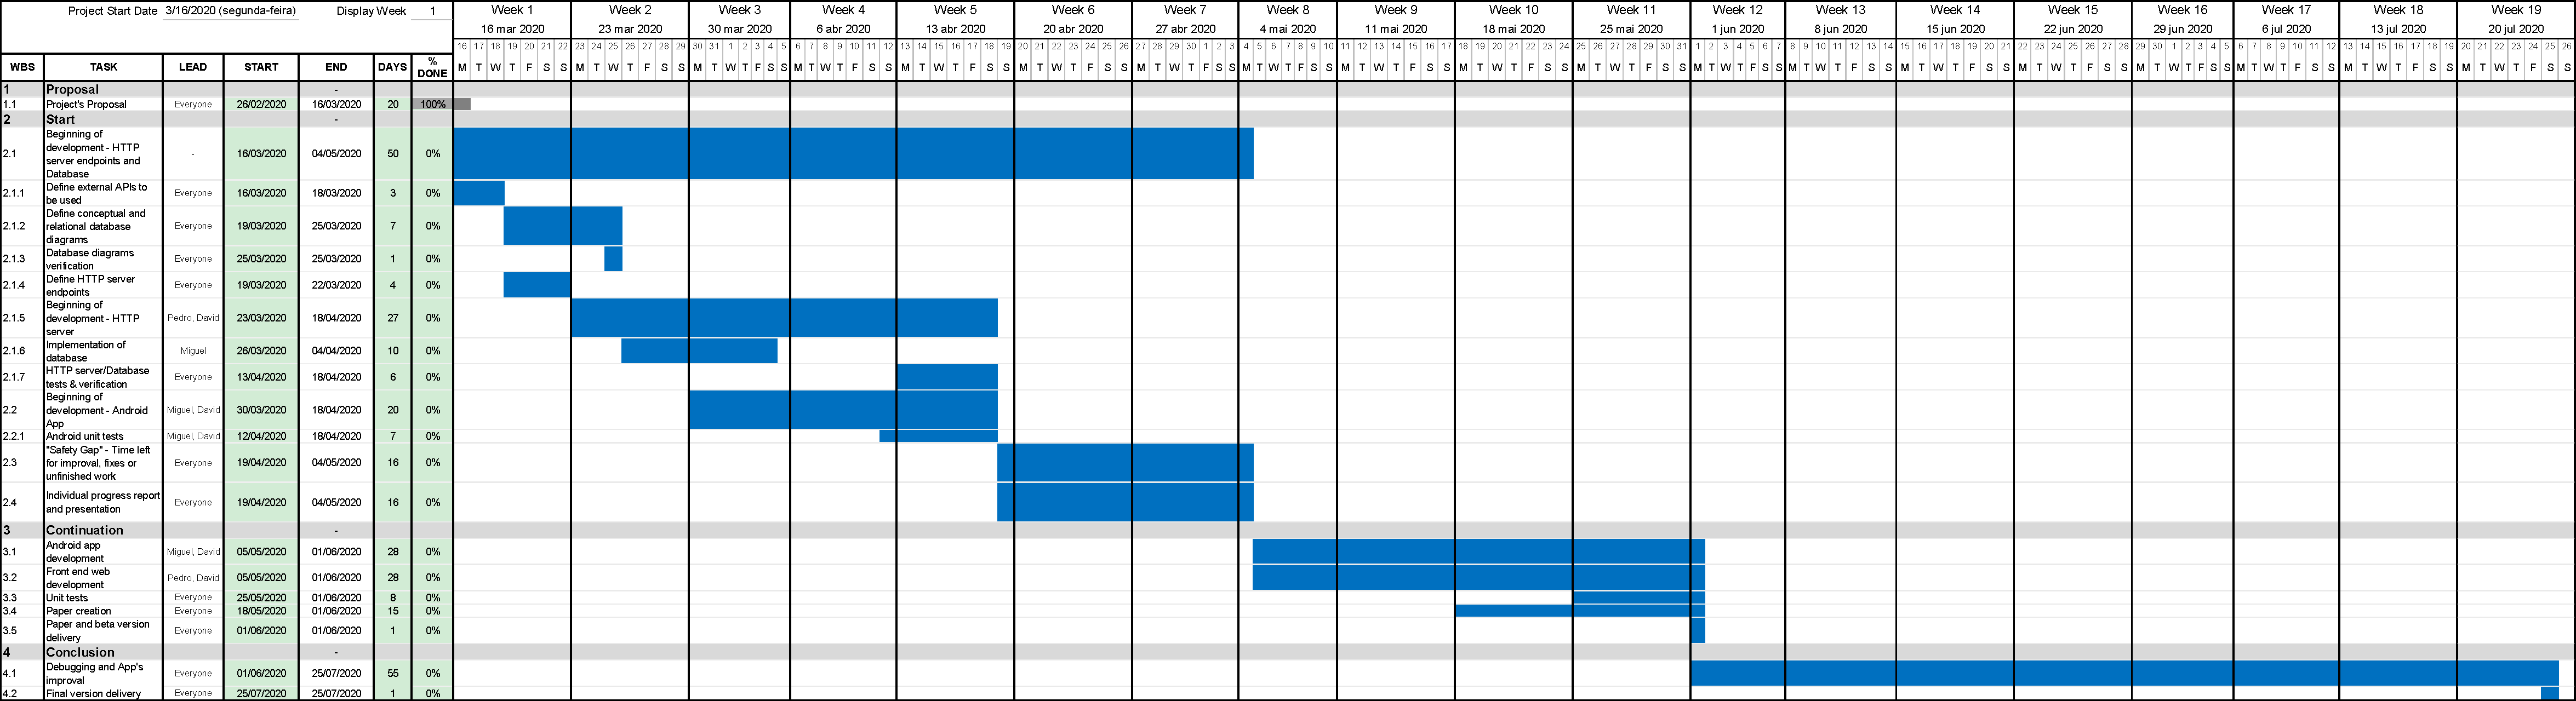
\includegraphics[scale=0.2]{pictures/Nutr.io project schedule.pdf}
    \caption{Nutr.io's initial project schedule (Vector format)}
    \label{fig:Nutr.io project's schedule}
\end{figure}

\begin{thebibliography}{15}

\bibitem{world}
\url{https://www.diabetesatlas.org/en/sections/worldwide-toll-of-diabetes.html.}

\bibitem{idf}
\url{https://www.idf.org/our-network/regions-members/europe/publications-and-resources/29-idf-europe-position-paper-on-mobile-apps.html}

\bibitem{myfitnesspal}
\url{https://www.myfitnesspal.com/}

\bibitem{stackoverflow}
\url{https://stackoverflow.com/}

\bibitem{heroku}
\url{https://www.heroku.com/}

\bibitem{googleplaces}
\url{https://developers.google.com/maps/documentation/}

\bibitem{zomato}
\url{https://developers.zomato.com/api}

\bibitem{yelp}
\url{https://www.yelp.com/developers/documentation/v3/get_started}

\bibitem{nutritionix}
\url{https://developer.nutritionix.com/}

\bibitem{react}
\url{https://reactjs.org/docs/getting-started.html}

\bibitem{singlepage1}
\url{https://rubygarage.org/blog/single-page-app-vs-multi-page-app}

\bibitem{singlepage2}
\url{https://docs.microsoft.com/en-us/dotnet/architecture/modern-web-apps-azure/choose-between-traditional-web-and-single-page-apps}

\bibitem{zomato1}
\url{https://developers.zomato.com/api/v2.1/dailymenu?res_id=18229073}

\bibitem{zomato2}
\url{https://developers.zomato.com/api/v2.1/dailymenu?res_id=18388621}

\bibitem{zomato3}
\url{https://developers.zomato.com/api/v2.1/dailymenu?res_id=8214729}

\end{thebibliography}

\end{document}
